\documentclass[draft,linenumbers]{agujournal2018}
\usepackage{apacite}
\usepackage{url} %this package should fix any errors with URLs in refs.
\usepackage{amsmath}
\usepackage{xcolor}
\usepackage[colorlinks]{hyperref}
\usepackage[colorinlistoftodos]{todonotes}

%\usepackage{framebox}

%%%%%%%
%\usepackage{trackchanges}
% uncomment the line above to use the TrackChanges package to mark revisions if needed.
% The trackchanges package adds five new LaTeX commands:
%
%  \note[editor]{The note}
%  \annote[editor]{Text to annotate}{The note}
%  \add[editor]{Text to add}
%  \remove[editor]{Text to remove}
%  \change[editor]{Text to remove}{Text to add}
%
% complete documentation is here: http://trackchanges.sourceforge.net/
%%%%%%%https://www.overleaf.com/project/5c3620127117e2522d9e0c30

\draftfalse

\journalname{Space Weather}

\begin{document}

% Not working
% \listoftodos

\title{A Test of the Frequency Independence Assumption of Power System Parameters used in Geomagnetically Induced Current Estimates}

\authors{R.S. Weigel\affil{1} and P.J. Cilliers\affil{2}}

\affiliation{1}{Space Weather Lab, George Mason University}
\affiliation{2}{South African National Space Agency}

\affiliation{1}{4400 University Drive, Fairfax VA 22030}
\affiliation{2}{Hospital Street, Hermanus 7200}

\correspondingauthor{R.S. Weigel}{rweigel@gmu.edu}

\begin{keypoints}
\item Power system parameters derived from a time series of GIC and geoelectric field measurements are frequency dependent.
\item A GIC prediction model with frequency dependent system parameters significantly outperforms a frequency independent model.
\item A model derived using GIC/geomagnetic field data provides better predictions than a GIC/geoelectric field-based model.
\end{keypoints}

\begin{abstract}
A common assumption used when estimating geomagnetically induced currents (GICs) in a power system given a nearby direct measurement or indirect estimate of the horizontal geoelectric field components $E_x(t)$ and $E_y(t)$ on Earth's surface is that the system is resistive. That is, the approximation $GIC(t)$  $=$ $a_oE_x(t) + b_oE_y(t)$ (Model 1) is used, where $a_o$ and $b_o$ are frequency independent network parameters.  A first test of this assumption is made using GIC measurements made in a 187 kV transformer connected to a $\sim$100~km power line in Memanbetsu, Japan and geoelectric field measurements made at the Memanbetsu Magnetic Observatory $\sim$9~km away.  Frequency-dependent network parameters $a(\omega)$ and $b(\omega)$ computed from data in Model 2, $GIC(\omega)$ $=$ $a(\omega)E_x(\omega) + b(\omega)E_y(\omega)$,  are shown to be frequency dependent and this model provides a significantly better estimates of the measured GIC over Model~1. A third model, which uses the electric field estimated by convolving a magnetotelluric transfer function with the geomagnetic field, provides significantly better estimates over Model~2. It is suggested that the measurement-derived frequency dependence of the system parameters is explained by spatial variations in the spectrum of the geoelectric field along the line in which GIC is measured rather than by an actual frequency dependence of the system parameters.
\end{abstract}

\section{Introduction}

Geomagnetically induced currents (GICs) are electric currents in conducting systems that are due to electric fields near the Earth's surface. Time-varying electric and magnetic fields at Earth's surface are driven by time variations in ionospheric currents on time scales on the order of hours \citep{Ohtani2000} and the movement of Earth's surface relative to slow-varying current systems in Earth's ionosphere that are near stationary relative to the Sun \citep{Stening2013}. Of particular interest are currents induced in electric power systems because they can lead to system degradation, disruption, and failure \citep{Albertson1993,NERC2012,Gaunt2014}. Accurate estimation of GIC magnitudes is important for power system design, retrospective analysis, and mitigation of the impacts of space weather on power systems \citep{Molinski2002,Thomson2010,NERC2012,Gaunt2014}. 

A common assumption made in estimates of GIC in an electric power system using either a measured or estimated time series of the horizontal geoelectric field at Earth's surface, $\mathbf{E}(t)$, is that the power system is resistive or quasi-DC in the sense that the relationship $GIC(t) = a_oE_x(t) + b_oE_y(t)$ holds \citep{Albertson1981,Lehtinen1985}. In this case, estimates of the coefficients $a_o$ and $b_o$ can be easily made from the data using linear regression when contemporaneous measurements of $GIC(t)$ and $\mathbf{E}(t)$ are available, or by using information about the connectivity of the power lines and values of the conductor and transformer resistances using DC circuit methods \citep[e.g.,][]{Boteler2014a,Boteler2014b}. This quasi-DC assumption has been used or stated in many GIC-related works, for example, \citet{Pulkkinen2007,Wik2008,Pulkkinen2010,Ngwira2011,Horton2012,Viljanen2012,Overbye2012,Marshall2013,Liu2014,Zheng2014,Watari2015,Bonner2017}. 

%\cite{Oyedokun2013a} developed a method to account for the finite inductive response time of transformers by taking the GIC predicted based on the quasi-DC assumption and then applying a piecewise-linear L/R filter derived from bench-scale transformer measurements, with a time constant dependent on load, to obtain an alternative estimate of GIC. 

%\todo[inline]{What can I conclude from \cite{Oyedokun2013a}? Mostly the thesis documents visual differences in time series traces with and without accounting for transformers.} 

In this work, we use a unique dataset in which time series measurements of $\mathbf{E}$ and the surface horizontal geomagnetic field, $\mathbf{B}$, were made near a site where GIC was being measured in an electric power system.  We first estimate the system parameters $a_o$ and $b_o$ from data using conventional methods, in which they are modeled as frequency independent. Then, we use a model in which the system parameters are allowed to be frequency dependent, compute the frequency dependence, and compare this model's ability to represent GIC with the traditional frequency-independent model. 

\section{Data}

The 1-second-cadence GIC data used span a total of 35 days across 10 intervals that start and end at midnight Japan Standard Time (JST): 2006-04-03 -- 2006-04-10, 2006-07-25 -- 2006-07-29, 2006-08-05 -- 2006-08-08, 2006-08-19 -- 2006-08-21, 2006-11-07 -- 2006-11-12, 2006-11-28 -- 2006-11-29, 2006-12-01, 2006-12-14 -- 2006-12-15, 2007-11-18 -- 2007-11-20, and 2007-11-22 -- 2007-11-22. These data have been presented previously in \citet{Watari2009} and \cite{Watari2015}. These time intervals are those for which GIC data was made available with the exception of three days for which there were obvious problems with either the electric field or GIC measurements. The GIC dataset includes 1~s raw data and 1~Hz low-pass-filtered raw measurements. The results presented here are for the 1~Hz low-pass-filtered GIC measurements

One-second-cadence $\mathbf{E}(t)$ and $\mathbf{B}(t)$ measurements from Memambetsu Magnetic Observatory were obtained from the Japan Meteorological Agency data portal.

Data for the time span of 2006-08-04T15:00 through 2006-08-08T15:00 are shown Figure~\ref{sample}. The GIC data were provided as 1-day files that start at midnight JST and the times shown in Figure~\ref{sample} are Universal Time.

Spikes in the electric field measurements were assumed to be unphysical when the absolute value of a component $i$ of the electric field changed by more than 1~mV/km at time $t_s$, and the values $E_i(t_s-2)$ through $E_i(t_s+4)$ were replaced using linear interpolation of the values at $E_i(t_s-3)$ and $E_i(t_s + 5)$. In the sample shown in Figure~\ref{sample}, 21 spikes were identified in $E_x$ and zero in $E_y$. For all of the time intervals considered, the fraction of interpolated $\mathbf{E}$ values ranged from 0--0.1\%.

The only modification made to the magnetic field measurements was the replacement of 36 data points on 2006-08-06 with linearly interpolated values. The 36 values for $B_x$ and $B_y$ were the same and much larger than the surrounding values.

The GIC data contains non-physical spikes that are followed by a relaxation time of 40-80 s. These spikes were removed by identifying times $t_s$ when the change in the 1~s absolute value of $GIC(t)$ was greater than $0.05$~Amps and then values in a window $GIC(t_s-2)$ through $GIC(t_s+100)$ were replaced using a linear interpolation of the values at $GIC(t_s-3)$ and $GIC(t_s + 101)$. In the example interval shown in Figure~\ref{sample}, 493 spikes were removed. For all of the time intervals considered, the fraction of interpolated GIC values ranged from 1--4\%.

\section{Models and Methods}

To determine the coefficients $a_o$ and $b_o$ in the frequency independent model, Model~1,

\begin{linenomath*}
\begin{equation}
G_o(t) = a_oE_x(t) + b_oE_y(t)
\label{model1}
\end{equation}
\end{linenomath*}

\noindent
the matrix equation $\underline{\mathbf{GIC}} = \underline{\mathbf{E}}\cdot\mathbf{p}$ is solved in a least squares sense, where $\underline{\mathbf{GIC}}$ is a zero mean 86400x1 matrix of 1 day observations with rows of $GIC(t)$; $\mathbf{p} = [a_o,b_o]^T$, and $\underline{\mathbf{E}}$ is a 86400x2 matrix with rows of $[E_x(t), E_y(t)]$ with zero mean columns. The values of $a_o$ and $b_o$ determined in this way correspond to those that minimize the sum-of-squares of $GIC(t)-G_o(t)$ over a 1-day interval. \citep[][provided the mathematically equivalent closed-form equations for solving the matrix equation.]{Pulkkinen2007} The notation $\overline{a}_o$ and $\overline{b}_o$ will be used for the average of the $a_o$ and $b_o$ values computed using the 35 1-day window segments of available data.

In Model 2, the system parameters $a(\omega)$ and $b(\omega)$ are frequency dependent according to

\begin{linenomath*}
\begin{equation}
G_E(\omega) = a(\omega)E_x(\omega) + b(\omega)E_y(\omega)
\label{model2}
\end{equation}
\end{linenomath*}
\noindent
and are computed using contemporaneous measurements of $GIC(t)$ and $\mathbf{E}(t)$. The method of parameter estimation and generating predictions for Models 2-4 are given at the end of this section and fourier transformed variables are indicated by explicitly listing their dependence on $\omega$.

In Model~3, the parameters $a(\omega)$ and $b(\omega)$ from Model~2 are used, but with an electric field $\mathbf{E}'$ computed using the measured magnetic field, $\mathbf{B}$, and a transfer function $\boldsymbol{Z}$: $\mathbf{E}'(\omega) \equiv \boldsymbol{Z}(\omega)\mathbf{B}(\omega)$ and

\setcounter{equation}{2}
\begin{linenomath*}
\begin{equation}
G_{E'}(\omega) = a(\omega)E'_x(\omega) + b(\omega)E'_y(\omega)
\label{model3}
\end{equation}
\end{linenomath*}

\noindent
where, explicitly, the electric field components are $E'_x$ = $Z_{xx}B_x + Z_{xy}B_y$ and $E'_y = Z_{yx}B_x + Z_{yy}B_y$. 
That is, instead of using the measured electric field directly as in Model 2, a magnetotelluric transfer function that relates $\mathbf{E}$ to $\mathbf{B}$ is used to provide an estimate of the electric field based on the magnetic field.

%Substitution gives

%\begin{linenomath*}
%\begin{equation*}
%G_{E'}(\omega) = %\big[a(\omega)Z_{xx}(\omega) + b(\omega)Z_{yx}(\omega) \big] B_x(\omega) + \big[ a(\omega)Z_{xy}(\omega) + b(\omega)Z_{yy}(\omega) \big] B_y(\omega)\,.
%\end{equation*}
%\end{linenomath*}

The fourth model is

\begin{linenomath*}
\begin{equation}
G_B(\omega) = z_x(\omega)B_x(\omega) + z_y(\omega)B_y(\omega)\,.
\label{model4}
\end{equation}
\end{linenomath*}

\noindent
In this model, the transfer function components $z_x$ and $z_y$ are determined directly from measurements of $GIC(t)$ and $\mathbf{B}(t)$ and no electric field measurements are used; this model is expected to produce predictions of GIC that are similar to that obtained from Model 3 because they both use the same input variable.

Estimates of $a(\omega)$ and $b(\omega)$ are made at evaluation frequencies, $\omega_e \equiv 2\pi f_e$, by performing a ordinary least squares regression (OLS) using Equation~\ref{model2} and a set $G_E(\omega)$ and $\mathbf{E}(\omega)$ values near $f_e$ from the DFT (discrete fourier transform) of 24 hours of 1-s cadence data. The 28 values of $f_e$ start at $0.25$ Hz and decrease by a factor of $\sqrt{2}$ and end at $1/43200$~Hz; if the $f_e$ value computed in this way is not an integer multiple of $1/86400$, the nearest smaller integer multiple is used. The regression for each $f_e$ uses all DFT frequencies with values in a window with a width of twice the separation from the next lower value of $f_e$ and the given $f_e$ with the exceptions that the lowest evaluation window has a lower bound of $1/86400$~Hz and highest evaluation window has an upper bound of $0.5$~Hz. 

The same approach is used for solving for $z_x$ and $z_y$ in Equation~\ref{model4}. For the transfer function $\boldsymbol{Z}$ in $\mathbf{E}(\omega) = \boldsymbol{Z}(\omega)\mathbf{B}(\omega)$ used in Model~3, the $xx$ and $xy$ components of $\boldsymbol{Z}$ are solved for using $E_x(\omega) = Z_{xx}(\omega)B_x(\omega) + Z_{xy}(\omega)B_{y}(\omega)$; the $yx$ and $yy$ components are solved for using $E_y(\omega) = Z_{yx}(\omega)B_x(\omega) + Z_{yy}(\omega)B_y(\omega)$.

Transfer function parameters were computed for each of the segments. The average transfer function magnitude and phase at a given evaluation frequency was obtained by averaging the segment values at that evaluation frequency.

To convert the frequency domain transfer function parameters estimated at the evaluation frequencies to impulse responses, their real and imaginary components are linearly interpolated individually onto the original DFT frequency grid (with spacing of $1/86400$~Hz), and then the inverse DFT is computed. The interpolated transfer function parameters were set to zero at frequencies higher than $0.25$~Hz and the transfer function estimate at $f=0$ was set to zero before interpolation.

Prediction time series were calculated by convolution of the interpolated transfer function parameters with the DFT of the 24-hr long and 1~s cadence model inputs and computing the inverse DFT (e.g, for Model~2, $G_E(f)=a^I(f)E_x(f)+b^I(f)E_y(f)$ was calculated, where the superscript $I$ indicates the interpolated value, and then the inverse DFT of $G_E(f)$ was calculated to give the prediction $G_E(t)$ on a 1~s time grid).

Several modifications to this basic procedure were considered. Robust regression \citep{Egbert1986} with a Huber weighting constant of $1.345$ and an upper limit of 50 iterations and bi-square weighting with a constant of $4.685$ (both constants provide 95\% efficiency for normally distributed errors), both with no hard-cutoff step; time domain pre-whitening and tapering; and weighting the frequencies around each evaluation frequency using Parzen window weights. When using these additional steps individually, we find that the conclusions made regarding the differences each model's prediction ability do not change because the differences in each model's prediction performance are within the calculated uncertainty of the used method. Transfer function parameter values found using these modifications are generally within the error bars of those for the used procedure when the signal to noise ratio is above $\sim$3 (corresponding to a period of $\sim 30$~s; At periods below $\sim$30~s, the electric field measurements are significantly influenced by the instrument response characteristics~\citep{Fujii2015}, aliasing, and the computed values are also expected to be significantly biased due to low signal to noise ratio.)

\section{Results}

The out-of-sample prediction metrics for each model on day $D$ were determined by computing the average model parameters using the remaining 34 days of data and then using these averaged parameters to generate a prediction time series and associated metrics on day $D$. This process was repeated to create a set of 35 out-of-sample prediction metrics for each model. In calculating the metrics, the first and last 10 minutes of the day were excluded to reduce the effect of transients that exist in the prediction at the start of the interval for the amount of time that the causal part of the impulse response is non-zero and at the end for the amount of time that the acausal part of the impulse response is non-zero. 

The performance of each model in predicting GIC was assessed using three metrics: the prediction efficiency, PE, the mean-squared-error (MSE) ratio, and the signal-to-noise ratio.

The prediction efficiency, PE, is the ``Case I'' skill score described by \cite{Murphy1988} and is defined as PE = 1 - variance(Prediction Error)/variance(Predicted); it is a measure of the skill of the model relative to the variance in the data that are predicted, and it represents the fraction of the variance in the data that predicted by the model.

The average PE and MSE ratios were computed by averaging the out-of-sample PE and MSE ratios; the average signal-to-noise ratio at a given frequency is the average of the out-of-sample signal-to-noise ratios at that frequency. The 95\% confidence interval, CI, on the PE and MSE ratio was calculated using 1000 bootstrap samples of the out-of-sample prediction metrics. (The typical difference between the limits when the confidence intervals were computed assuming the values were Gaussian-distributed was $\sim$2\%.) The spectra for the signal and prediction error for each of the segments at a given evaluation frequency was obtained by averaging the raw spectra using the same frequency windows used for the regression. 

\begin{table}
\caption{Out-of-sample model performance metrics for models $m=1-4$. MSE$_m$/MSE$_1$ is the ratio of the MSE for model $m$ to that of Model 1. The PE and MSE ratios are the average of 35 values and the confidence interval, CI, was determined from 1000 bootstrap samples.}
\centering
\begin{tabular}{l c c c c}
\hline
$m$\hspace{1em} Model & PE & 95\% CI & MSE$_m$/MSE$_1$ & 95\% CI\\
\hline
1\hspace{1em} $G_o(t) = a_oE_x(t) + b_oE_y(t)$ & 0.35 & [0.25, 0.45] & 1.0 & \\
2\hspace{1em} $G_E(t) = a(\omega)E_x(t) + b(\omega)E_y(t)$ & 0.60 & [0.54, 0.65] & 1.8 & [1.6, 2.0]\\
3\hspace{1em} $G_{E'}(t) = a(\omega)E'_x(t) + b(\omega)E'_y(t)$ & 0.78 & [0.76, 0.80] & 3.1 & [2.8, 3.4]\\
4\hspace{1em} $G_{B}(t) = Z_xB_x(t) + Z_yB_y(t)$ & 0.83 & [0.80, 0.85] & 4.6 & [3.8, 5.3]\\
\hline
\end{tabular}
\end{table}

Figure~\ref{predictions} shows the predictions for each model in a 1-day interval selected because the value of the prediction efficiency for each model was in the same order as that shown in Table~1, i.e., Model 1 has the lowest PE and Model 4 has the highest.

The primary conclusions of this work follow from the results shown in Table~1: the frequency dependent model, Model~2, is significantly better at predicting GIC than the frequency independent model, Model~1; Model~3, which uses an estimate of the electric field based on magnetic field measurements, provides significantly better estimates of GIC than Model~2; Model~4, in which a transfer function that connects GIC to $\mathbf{B}$ was derived directly from the data, provides better estimates of GIC than Model~3.

To determine the statistical significance, $10^5$ bootstrap averages of the PEs of each model were created and their differences were computed. From this, the null hypothesis that the PE of Model~2 is equal to that of Model~1 can be rejected at a significance level of less than $10^{-5}$ because the bootstrap average of Model~2 was not found to be lower than that for Model~1. The null hypothesis that the PE of Model~3 is equal to that of Model~2 can also be rejected at the same significance level. The null hypothesis that the PE of Model~4 is equal to that of Model~3 can be rejected at a significance level of $10^{-2}$.

%Although inferior, the Model~1 does have a good prediction performance - the PE is 0.35 and the data/model correlation coefficient of 0.64. The top panel of  Figure~\ref{predictions} shows that its predicted GIC generally follows the overall trend of the measured GIC.

Figure~\ref{SN} shows the average signal-to-noise (i.e., signal to prediction error) ratios as a function of period for the four models. At each evaluation frequency, the SN ratio is the ratio of the average of the out-of-sample SN ratios of the segments and the error bars represent a 95\% CIs based on 1000 bootstrap samples of the segment SN ratios. 

Consistent with the results in Table~1, The SN ratio for Model~1 is lower than that for Models~2-4 at all frequencies. However, ordering of the SN ratio for Models~2-4 is dependent on period. 

Below $600$~s (10~min), Model~2 has the largest SN ratio. This result is somewhat visible in the sample interval shown in Figure~\ref{predictions} where the high-frequency fluctuations in the prediction error for Model~2 are the smallest among the models. For these periods, the predictive ability of each model is in the order that may be expected based on the data used to derive the model: Model~2, which uses direct measurements of the electric field, has a higher SN ratio than Model~3, which uses an indirect estimate of the electric field. Model~4 has a slightly higher SN than Model~3, and this is expected because they both use the same input of the magnetic field, but Model~3 has an additional source of uncertainty from the parameters in $\mathbf{Z}$. Above $600$~s, the ordering of the SN is not consistent with these expectations and is possibly explained by two factors (1) the measured GIC is based on an integrated electric field along the power line, and the electric field used in Model~2 is a point measurement - the result is that implicit in the model is an assumption that the electric field is uniform over the length of the line on which GIC is measured and (2) the error associated with this assumption has less of an influence on the errors in a model that uses the point measurements of the magnetic field. Issues related to this are discussed in the following section.

Above $10,000$~s (2.8~hrs), the SN ratio ordering is the same as the ordering of the PE and MSE ratios shown in Table~1, with Model~1 having the lowest and Model~4 having the highest SN ratio. 

The average parameters and 95\% CI for Model 1 are $a_o = 73$ $[62,83]$ A/(V/km) and $b_o = -72.0$ $[-98,-45]$ A/(V/km) and the distribution of the parameters for the segments is shown in Figure~\ref{histogram}. (Results are similar if 1-minute averages are used; \cite{Watari2015} found $a_o=38.1$ A/(V/km) and $b_o=-7.4$ A/(V/km) for the interval 2006-12-14--2006-12-15 JST time interval). 
 
%However, for the data considered in this work, when a model $G(t) = $ $c_oB_x(t) + d_oB_y(t)$ is used, were $c_o$ and $d_o$ are constants, the in-sample average prediction efficiency is comparable to that of Model 1, but the out-of-sample prediction efficiency is negative.

The average parameters for Models~2 and~4 are shown in Figure~\ref{H}--\ref{Phi}. The error bars at each time step or period is the standard error of the 35 values used to compute the average.

%Figure~\ref{H} shows that the timescale of variations of an impulse in $\mathbf{E}$ for Model~2 and $\mathbf{B}$ for Model~4 are similar and are different from zero at more than one time value (the impulse response for Model~3 is similar to that of Model~2 and is not shown). By definition, the impulse response for Model~1 is zero except at $t=0$. Note that the sign of the $E_y$ impulse response at $t=0$ for Model~1 is opposite that for Model~2 (at $t=0$, $b_o < 0$ while $h_b(t=0)>0$). (An explanation for the acausality of the impulse response is given in \cite{Egbert1992,Kelbert2017}).

Figure~\ref{Z} shows that the frequency domain transfer functions for Model~2 vary by an order of magnitude on timescales of 60~s to 12~h (that for Model~1 is constant by definition). For this system, GIC more sensitive to $E_y$ than $E_x$ due to $b(\omega) > a(\omega)$, but note that $E_y(t)$ has less variability than $E_x(t)$ - the variance in $E_x(t)$ is $\sim$5x larger than $E_y(t)$ over the entire dataset (this is also visible in Figure~\ref{sample}). The ratio of $|\overline{b}_o|/|\overline{a}_o|$ is approximately 1 for Model~1 and this can be compared with $|b(\omega)|/|a(\omega)|$ calculated using the lines for $|a(\omega)|$ and $|b(\omega)|$ shown in Figure~\ref{Z}. The ratio varies from 2.7 at $T=30$~s to 1.6 at $T=12$~h. At $T=12$~h, the highest period considered, the phases of $a(\omega)$ and $b(\omega)$ shown in Figure~\ref{Phi} differ by 180 degrees and the signs are consistent with $\overline{a}_o$ and $\overline{b}_o$. 

Figure~\ref{Phi} shows the transfer function phases (that for Model~1 is 0$^o$ for positive parameters and 180$^o$ for negative parameters by definition). The phases for $z_x(\omega)$ and $b(\omega)$ are offset by 120$^o$ while the phases for $a(\omega)$ and $b(\omega)$ are significantly different.

%\cite{Pulkkinen2010} noted that one could estimate the ratio of $a_o/b_o$ using GIC and local geomagnetic field measurements even if $\mathbf{Z}(\omega)$ was unknown if one assumed the ground conductivity was 1-D so that $Z\equiv Z_{xy}=-Z_{yx}$ and $Z_{xx}=Z_{yy}=0$ so that Equation~\ref{model2} can be written

%\begin{linenomath*}
%\begin{equation}
%G(\omega) = a_oZ(\omega)B_y(\omega)/\mu_o - b_oZ(\omega)B_x(\omega)/\mu_o\,.
%\label{pulkkinen2010}
%\end{equation}
%\end{linenomath*}

%\noindent
%If the above equations are solved for with unknowns $Z_a\equiv a_oZ$ and $Z_b\equiv b_oZ$,  then $a_o/b_o = Z_a(\omega)/Z_b(\omega)$. \cite{Pulkkinen2010} assumed that this ratio was frequency independent and provided a closed-form equation for $a_o/b_o$ by multiplying Equation~\ref{pulkkinen2010} by the complex conjugates of $B_x(\omega)$ and $B_y(\omega)$ so as to form two equations from which $Z$ can be eliminated. With the additional assumption that the cross- and auto-spectra of all variables have the same functional form, they showed that the ratio can be written in a way that requires only evaluation of correlations among $G(t)$, $B_x(t)$, and $B_y(t)$.

\section{Discussion}

There are at least three possible explanations for the frequency dependence of the data-derived system parameters: (1) the quasi-DC approximation is invalid, (2) it is an artifact of the measurement process, and (3) the electric field is not spatially and spectrally constant across the region of the power system. 

(1) When the quasi-DC approximation is used, \cite{Albertson1981} is usually cited; their justification for the quasi-DC approximation is given the Appendix where it is stated that ``An analysis based on Carson's equations reveals that transmission lines can be modeled for GIC determination by using their positive sequence resistance values with a small correction factor to account for skin and proximity effects. The correction factor varies from 0.95 to 1.0 depending on conductor size.'' (Carson's equations  \citep{Carson1926,Grigsby2007} are equations for the impedance associated with a wire above an infinite and uniform half-space conducting slab.) \cite{Lehtinen1985} justifies the use of the quasi-DC approximation using the argument that GIC amplitudes are significant at frequencies that are much lower than the 50~Hz power line frequency. Clarified, this is essentially a statement that the reactance is proportional to frequency and although the reactance is $\sim$5 times larger than the resistance at 50~Hz \citep{Purchala2005}, the reactance will be $\sim$10 times smaller or less than the resistance at GIC frequencies of $\sim$1~Hz and lower. Given these arguments, the quasi-DC approximation is justified, and an explanation involving a violation of the assumption of a uniform half-space conducting slab Earth using a conductivity that varies with depth also seems unlikely to explain the results as it would need to account for at least an order of magnitude of reactance.

(2) A second consideration is that artifacts of the electric field and GIC measurements used in Model~2 cause the observed frequency dependence. However, the response characteristics of electric and magnetic field instruments are essentially frequency independent relative the observed frequency dependence for periods in the range considered of $10-10^{5}$~s \citep{Simpson2005} and the GIC instrument (HIOKI 9279 current sensor) is frequency independent to within $\pm 0.2$\% in this period range.

(3) The equation of Model~1 assumes that the electric field is spatially uniform at all points in the systems. The exact calculation of GICs in a power system under the quasi-DC assumption requires knowledge of the earth potential at the grounding points of the system, and simulations of GIC flow \citep{Albertson1981,Lehtinen1985} typically start with an assumed electric field along the lines to calculate these potential differences. The potential differences are then used along with the DC system component resistances and their connectivity to calculate GIC in the different parts of the system. In both Model~1 and Model~2, the input electric field is assumed to be spatially uniform along the line in which GIC was measured so that the potential difference is directly proportional to the electric field. If it is not, the parameters derived from the data in both models may differ significantly from those calculated using system configuration and resistance information. However, the data-derived parameters will not have a frequency dependence that results from a variation in the direction of the electric field along the line.

The second assumption of Model~1 is that the spectrum of the electric field is uniform. Violation of this assumption can lead to an apparent violation of the quasi-static approximation. Suppose the electric field and GIC are measured at one end of a long line segment and the electric field is non-zero only at a frequency of $\omega_1$. If the electric field is spectrally uniform along the full line segment, then from the quasi-static approximation it follows that the measured GIC will also only be non-zero at a frequency of $\omega_1$. If the electric field on the far half of the line is non-zero only at a frequency of $\omega_2$, the observed GIC and electric field will appear to be inconsistent with the quasi-static approximation because GIC will have non-zero variations at both $\omega_1$ and $\omega_2$.

To test the effect of different points on the line having different electric field spectra on the parameter estimates, we created a simulated GIC signal using electric field measurements made in Memambetsu (indicated with a superscript M) and Kakioka (superscript K), Japan:

\begin{equation}
G_s(t)=a_o\big[(1-r)E^{\mbox{\tiny M}}_x(t) + rE^{\mbox{\tiny K}}_x(t)\big]+b_o\big[(1-r)E^{\mbox{\tiny M}}_y(t) + rE^{\mbox{\tiny K}}_y(t)\big]
\end{equation}

\noindent
with $a_o=1$, $b_o=-1$ and $r=0.2$. $G_s$ represents a simulated GIC in which 20\% of the line has a different electric field. (The zero-lag correlation is -0.40 for $E^{\mbox{\tiny M}}_x(t)$ and $E^{\mbox{\tiny K}}_x(t)$ and 0.64 for $E^{\mbox{\tiny M}}_y(t)$ and $E^{\mbox{\tiny K}}_y(t)$). The model equation
\begin{equation}
G_s(\omega)=a(\omega)E^{\mbox{\tiny M}}_x(\omega)+b(\omega)E^{\mbox{\tiny M}}_y(\omega)
\end{equation}
\noindent
was then used to compute $a(\omega)$ and $b(\omega)$ and they were both found to exhibit a frequency dependence similar to that shown in Figure~\ref{Z} in that they both have an increase in magnitude by a factor of 2-6 for periods in the range of $2$~s to $12$~hr.

Although this proof-of-concept simulation shows how variations in the frequency content of the geoelectric field on the line in which GIC is measured can cause the data-estimated system parameters to have a frequency dependence, it is very crude as it uses several approximations that were necessitated by data availability. The distance from Kakioka to Memambetsu of $\sim$1400~km is $\sim$14x than the length of the power line of $\sim$100~km on which GIC was measured, and the correlations between the electric field from the two sites are likely to be lower than the fields measured at points separated by a distance closer to the length of the power line. In addition, the discontinuous change in the electric field implicit in the model does not satisfy Maxwell's equations and thus is not physically realizable. A more realistic simulation would use electric field measurements that were both near a line on which GIC was measured and separated from each other by a distance that is comparable to the length of the line.

%In the case that $E^{MMB}_x(t) = E^{KAK}_x(t)$, our calculation would give a frequency independent $a$.

%The violation of the spectral uniformity assumption may contribute to the explanation of the finding that Model~4 provides significantly better estimates of GIC than Model~1. On average, the magnetic field is more uniform spectrally than the electric field and so the parameters of Model~4 may be capturing both an MT response and spectral averaging effect.

%This explanation may also explain the finding that Model 4 provides significantly better predictions than Model 2 at long periods (but not at short periods). The magnetic field spectra typically exhibit significantly less spatial variability so the computed model parameters are able to capture a spatial averaging effect in addition to the effect of the ground impedance. 

%One way to test this hypothesis is to consider time intervals in which the spatial variability in the spectra of $\mathbf{E}$ is low -- the frequency dependence of $a(\omega)$ and $b(\omega)$ should be less than average. The frequency dependence of $a(\omega)$ and $b(\omega)$ should depend on the average spatial gradient in $\mathbf{E}_x(\omega)$ and $\mathbf{E}_y(\omega)$, respectively. (A reasonable test of this is not possible with this dataset because the nearest electric field instrument is $\sim$10x farther away from MMB, in Kakioka, Japan, than the length of the power line on which GIC was measured.)

%The finding that at long periods, the ratio of $a(\omega)/b(\omega)$ approaches $|\overline{b}_o/|/|\overline{a}_o|$

\section{Conclusions}

The primary implications of the results presented are (1) significantly improved predictions of GICs using data-derived system parameters $a$ and $b$ can be made if they are allowed to be frequency dependent and (2) a direct comparison of data-derived $a$ and $b$ parameters and those computed using power system configuration information will be problematic if the data are not consistent with the assumptions of Equation~\ref{model1}. 

Although the use of frequency independent $a$ and $b$ parameter values estimated from data give a reasonable out-of-sample prediction model, it is not known how much data-estimated parameter values will differ from those directly calculated. (Because the details of the power system under consideration in this work are not available, we were not able to make this comparison.) Works that use Model~1 and generally note a high degree of visual consistency between the measured values and predictions using this model (e.g., the top panel of Figure~\ref{predictions}). However, we have shown using a data set of contemporaneous GIC and $\mathbf{E}$ measurements that a significantly better estimation of GIC can be obtained by using a frequency dependent model of the form of Model~2. 

%The out-of-sample prediction quality reported here for Model~1 (a PE of 0.35 and CC of 0.64). If only a few days of data are used for their estimation, the out-of-sample prediction quality using all data is very poor due to the high degree of uncertainty of in their estimates \todo{Give example}. As a result, predictions of GIC using Model~1 in the literature using only a few days of data are expected to be significantly worse if out-of-sample predictions had been used.

When GIC and magnetic field measurements are available, a model of the form of Model~4 can be used. For this particular data set, we have found that such a model provides the best estimates of GIC in terms of the PE and MSE metrics. Local ground magnetic field estimates along with GIC measurements could be used to derive a transfer function model that is updated when the system configuration changes and this model could be used to estimate GIC under extreme or simulated geomagnetic conditions. A key advantage of this approach is that long-term geomagnetic field measurements are generally easier to make and are more readily available. A disadvantage is the transfer function parameters are difficult to interpret physically because they contain components of the transfer functions that connect $\mathbf{E}$ to $\mathbf{B}$ and GIC to $\mathbf{E}$ and frequency dependent artifacts due to violations of the assumption that the field is spectrally uniform.

%Based on the results in this work, the model of the form $GIC(t)$ $=a_oE_x(t)+b_oE_y(t)$, where the electric field is either measured or estimated using a transfer function at a given point near where GIC was measured, should be regarded as an approximation similar to that assumed when an equation of the form $GIC(t)$ $=c_oB_x(t)+d_oB_y(t)$ or $GIC(t)$ $=c_odB_x(t)/dt+d_odB_y(t)/dt$ is used, where $a_o, b_o, c_o, $and $d_o$ are constants (e.g., {\color{red} \textbf{[REFS]}}).

%Several methods have been used in the literature for estimating or predicting GIC depending on the data or models that are available.

%In addition, we have found that the estimates of the system parameters $a_o$ and $b_o$ are highly sensitive to the interval of data used, and have a high degree of uncertainty.

%When only a MT impedance tensor that connects $\mathbf{E}$ to $\mathbf{B}$ is available, a model of the form of Model~3, with the electric field estimated using $\mathbf{E}=\mathbf{Z}\mathbf{B}$ has been used~\citep{Marshall2013,Weigel2017,Bonner2017,Kelbert2017}. For the data set considered, significantly better GIC estimates can be made if frequency dependent system parameters are available. When the electric field $\mathbf{E}'$ is used in Model~1, the PE is X. \todo{Calculate X}


%~\ref{pulkkinen2010} used a variation of this approach but used an assumed conductivity model to estimate the frequency independent system parameters. 

%The frequency dependence of $a(\omega)$ and $b(\omega)$ shown in Figure~\ref{model2} is not consistent with a simple model of an ideal resistor $R$ in series with an ideal inductor $L$, for which the transfer function magnitude is $R^{-1}(1+\omega^2\tau^2)^{-1}$ and phase is $\tan^{-1}\omega\tau$, where $\tau=L/R$. 

%\todo{All - Need help in discussing the origin of the frequency dependence of the system parameters.}

%Ideally, frequency dependent system parameters could be calculated analytically for comparison with those estimated using data in this work. Because the details of the power system under consideration in this work are not available, we were not able to make this comparison. Note that frequency independent system parameters calculated using the approach in this work may not be directly comparable to those found from a network analysis for several reasons: (1) At periods less than $\sim 30$~s, the signal-to-noise ratio is low and the parameter estimates are expected to be biased; as shown in the Appendix, the transfer function estimates are highly sensitive to the method used for their calculation at (2) Also at periods less than $\sim 30$~s, effects of the instrument response may be significant. \cite{Fujii2015} has noted that the 1-s geoelectric field data from the Memambetsu Observatory were low-pass filtered with a 3.3-s cutoff-period prior to 2010; (3) The GIC observed in a power system is based on the integration of the electric field along a power line. All of the models assume that the electric field is constant along the line where the GIC is measured, but many works have shown that the electric field is expected to have variations on length scales comparable to the line considered ($\sim$100~km). \todo{REFS}

\acknowledgments
Magnetic and electric field data made at the Kakioka Magnetic Observatory was obtained from the Japan Meteorological Agency data portal \url{http://www.kakioka-jma.go.jp/obsdata/metadata/en}. We would like to thank the Hokkaido Electric Power Co. for the GIC measurements at the Memanbetsu substation and Shinichi Watari for communicating and preparing the GIC data and providing feedback on the manuscript. 
%\clearpage

\begin{figure}[h]
\centering
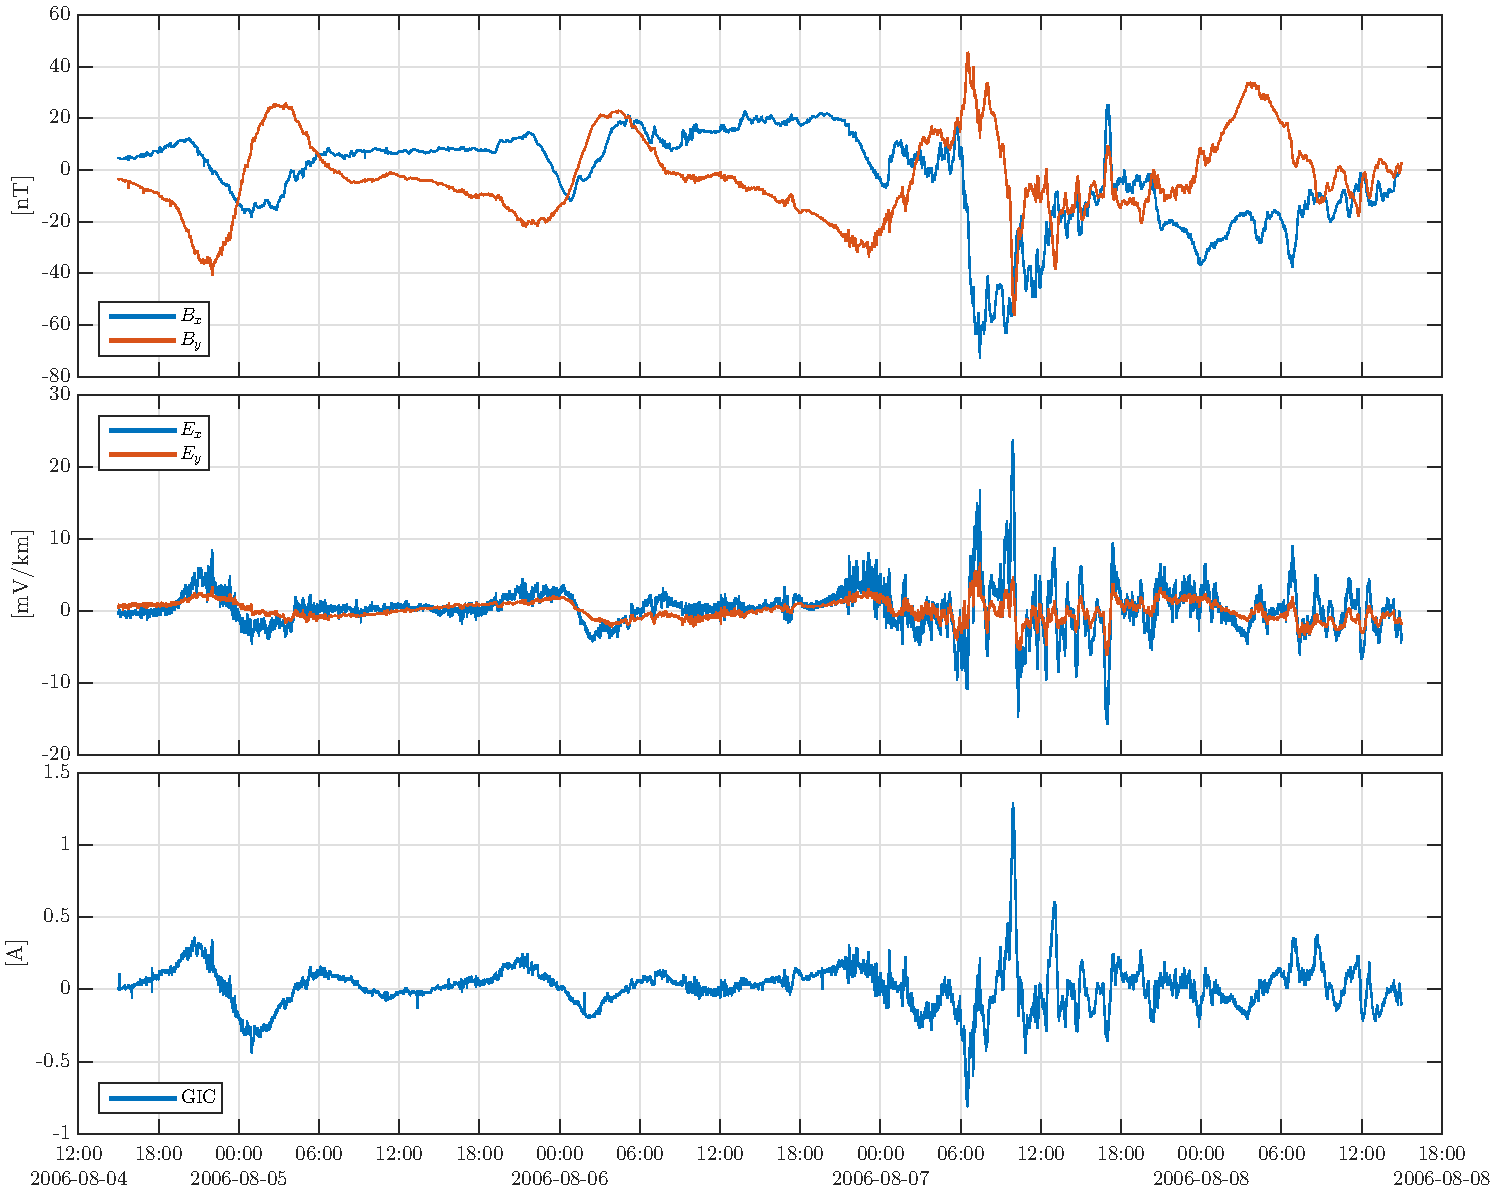
\includegraphics[width=\textwidth]{figures/plot_raw_All_20060805.pdf}
\caption{(Top) One-second-cadence geomagnetic field measured at the Memanbetsu Magnetic Observatory (MMB). (Middle) One-second-cadence geoelectric field measured at the Memanbetsu Magnetic Observatory (MMB) $\sim$9 km from the Memanbetsu substation. (Bottom) One-second-cadence GIC measurements measured in a grounded neutral point of a Y-connected three-phase transformer connected to a 187 kV bus at the Memanbetsu substation of the Hokkaido Power Co. The subscripts $x$ and $y$ correspond to Geographic North and East, respectively.}
\label{sample}
\end{figure}

\begin{figure}[h]
\centering
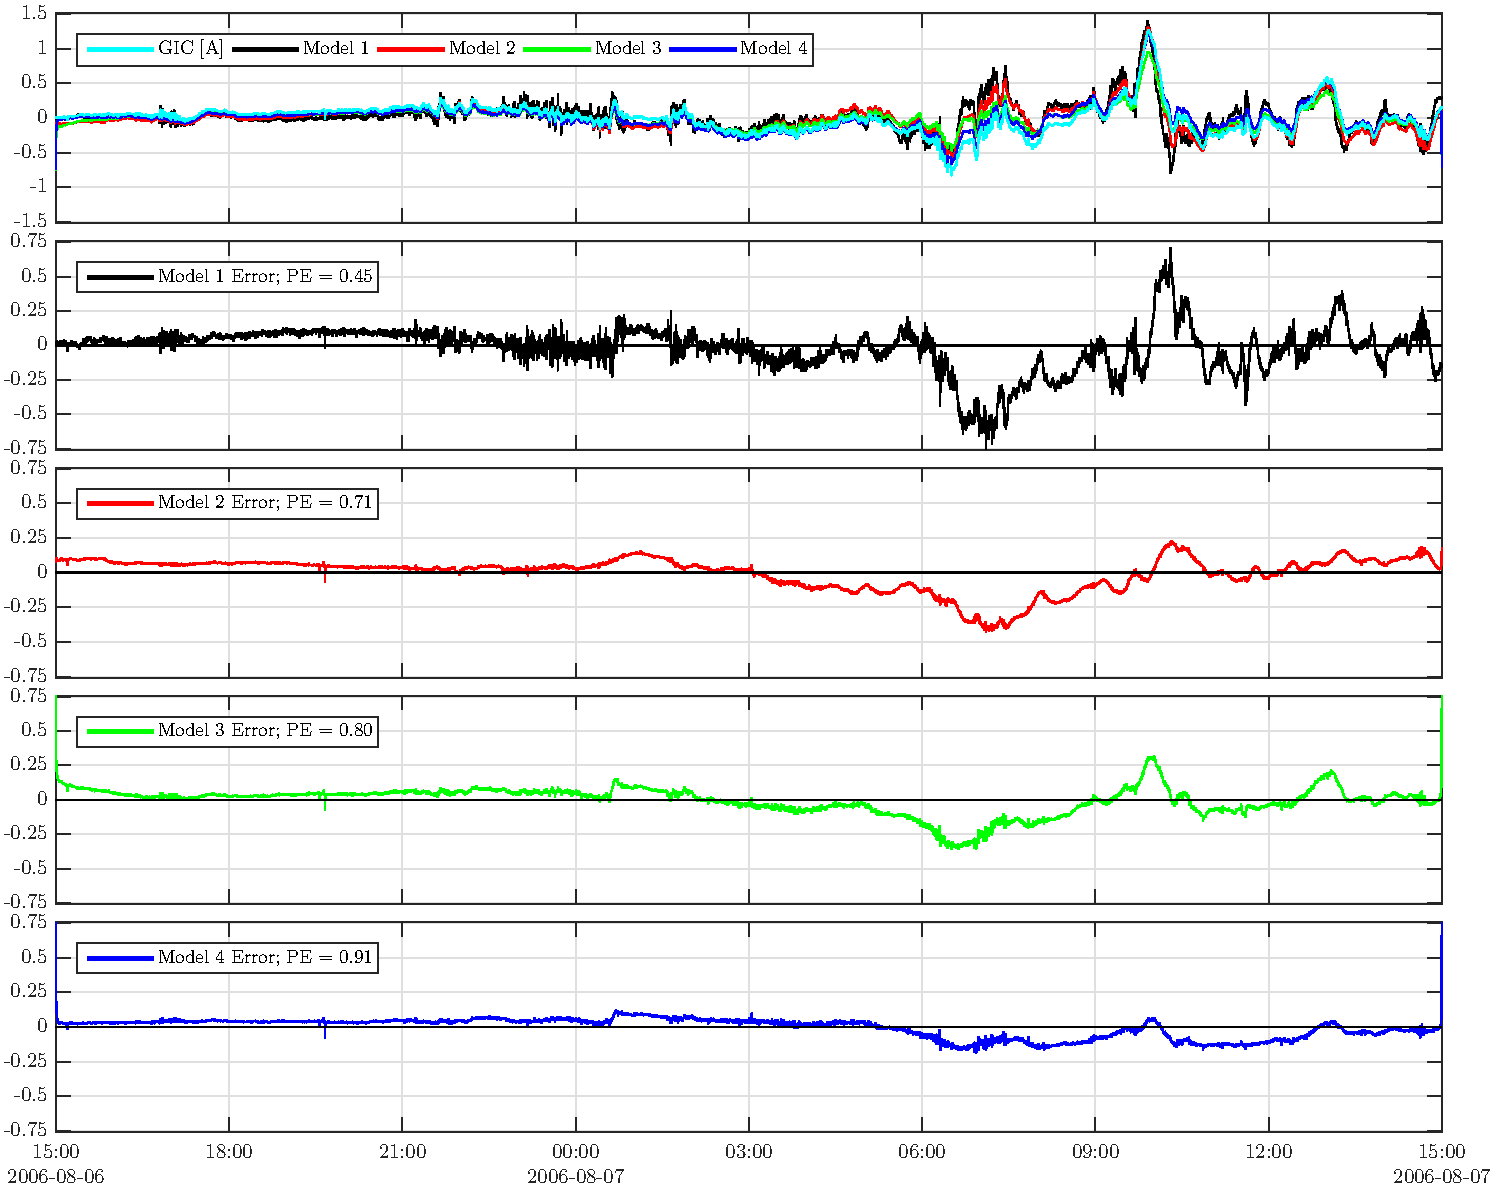
\includegraphics[width=\textwidth]{figures/plot_model_predictions-MeanModel-2006-08-06.pdf}
\caption{Out-of-sample model predictions (top) and predictions errors for a 1-day interval. Note that the scales for the error time series differ from that for the top panel so that the error amplitudes are scaled by a factor of 2.}
\label{predictions}
\end{figure}

\begin{figure}[h]
\centering
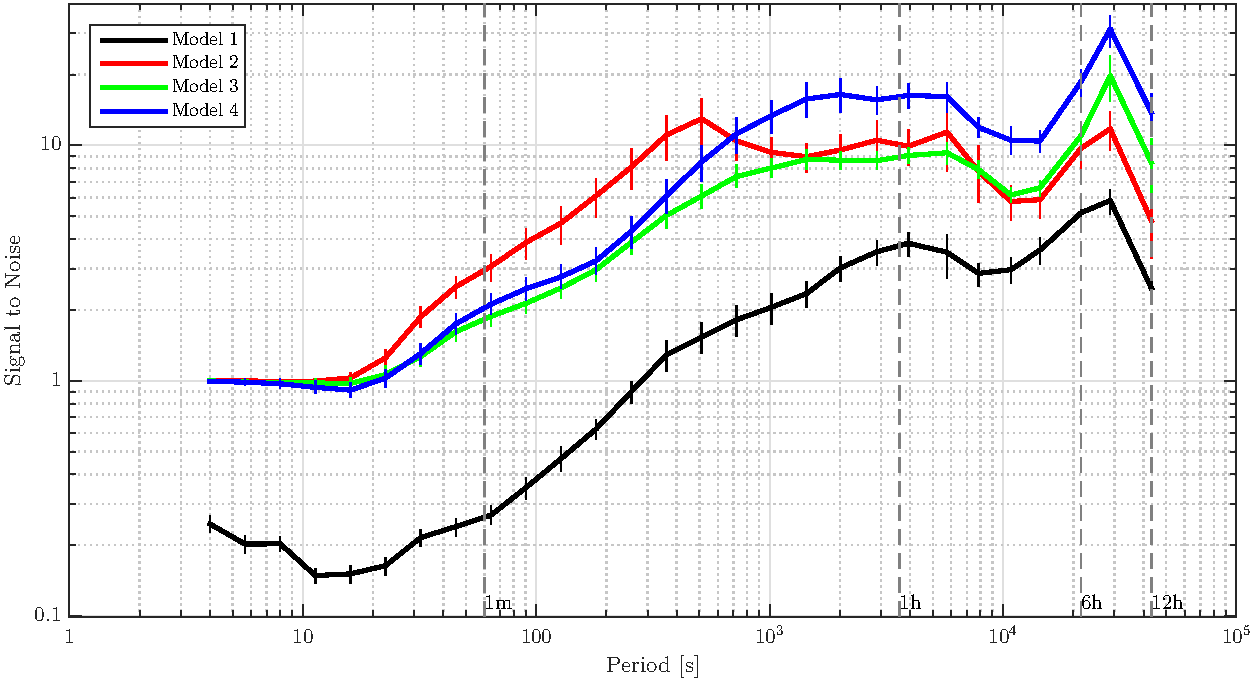
\includegraphics[width=\textwidth]{figures/plot_model_summary_SN-options-1.pdf}
\caption{Out-of-sample signal-to-noise (signal to prediction error) ratios at the evaluation frequencies for the four models.}
\label{SN}
\end{figure}

\begin{figure}[h]
\centering
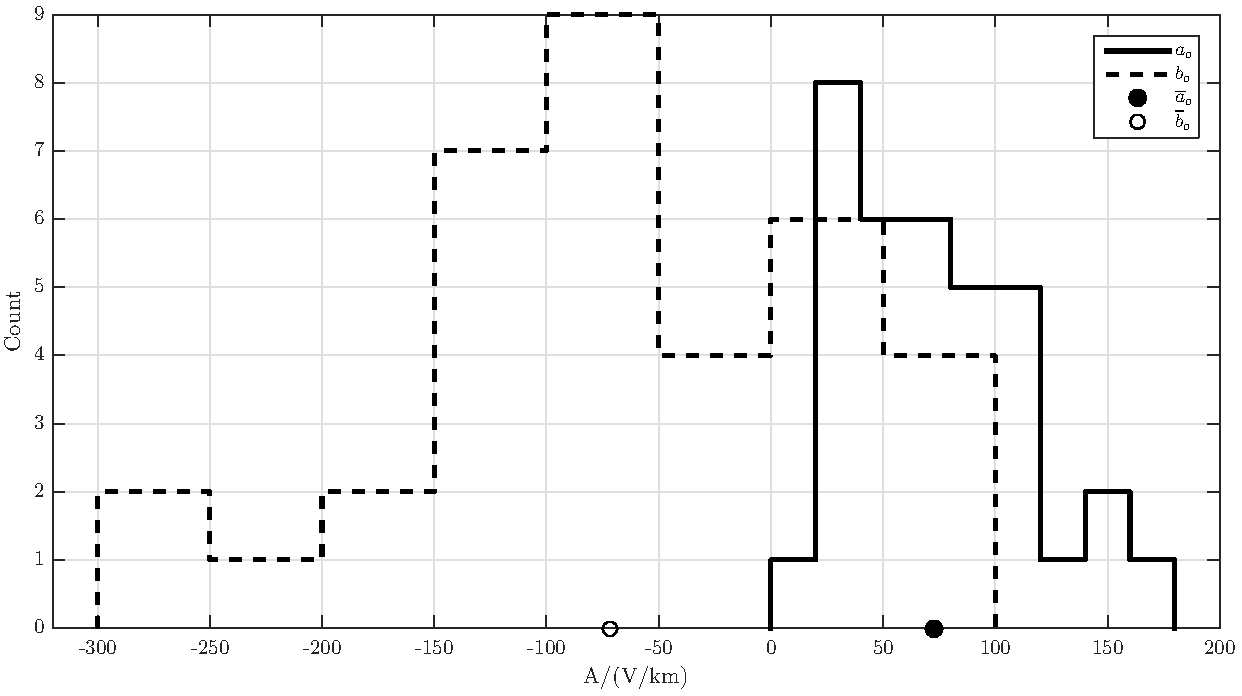
\includegraphics[width=\textwidth]{figures/plot_model_summary_aobo_histograms-options-1.pdf}
\caption{Distribution of parameters in Model 1. Each set of parameters was computed 35 times using one day of 1-second cadence data. The circle/dot on the horizontal axis indicates the average of each histogram: $a_o$ = 73 A/(V/km) and $b_o$ = -72.0 A/(V/km).}
\label{histogram}
\end{figure}

\begin{figure}[h]
\centering
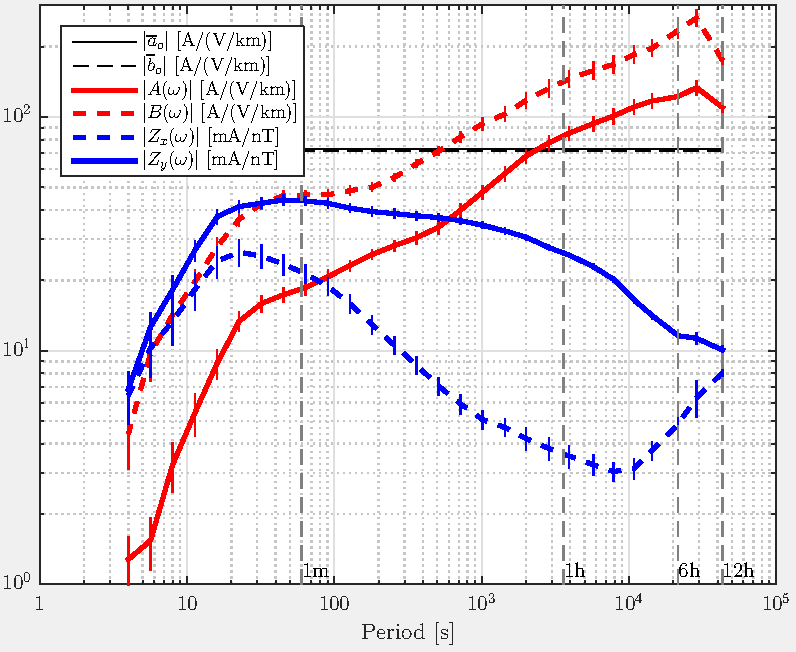
\includegraphics[width=\textwidth]{figures/plot_model_summary_Z-options-1.pdf}
\caption{Frequency domain transfer functions for the parameters in Models 1, 2, and 4. The frequency domain transfer functions for $a_o$ and $b_o$ in Model~1 are constant and equal to $a_o$ and $b_o$.}
\label{Z}
%\end{figure}

\vspace{4em}

%\begin{figure}[h]
\centering
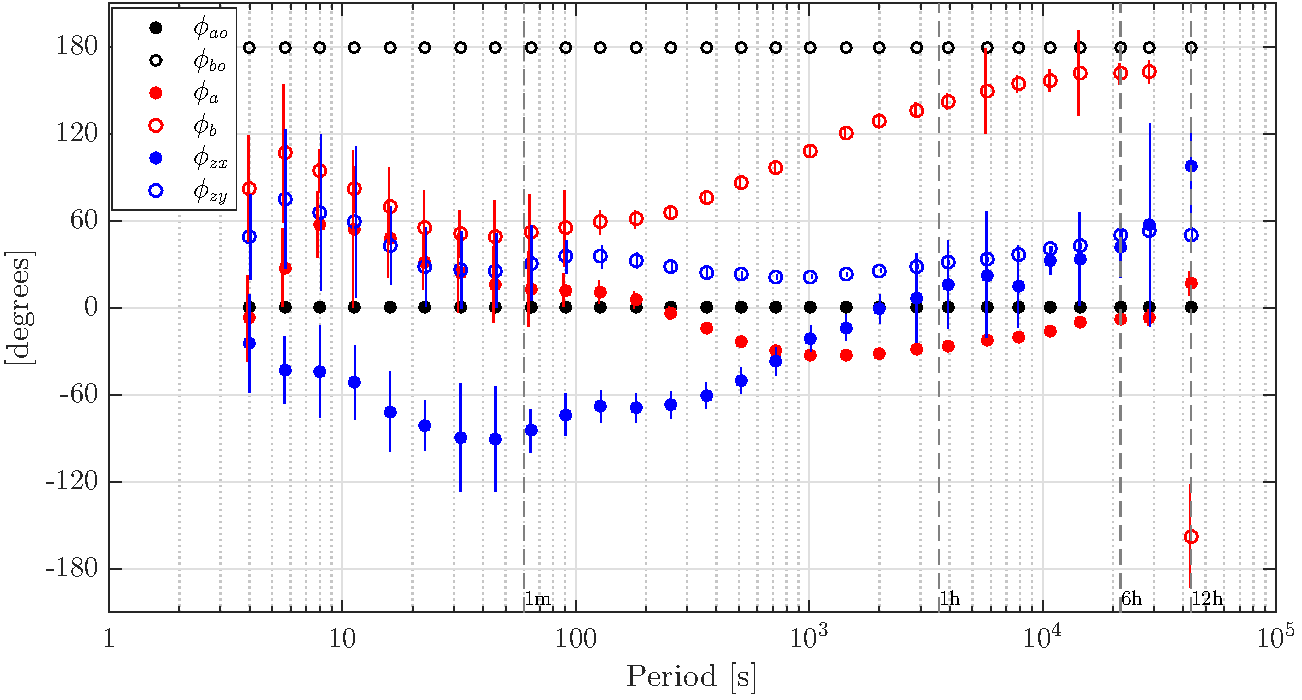
\includegraphics[width=\textwidth]{figures/plot_model_summary_Phi-options-1.pdf}
\caption{Frequency domain phase values for the parameters in Models 1, 2, and 4. The phase for $a_o$ and $b_o$ are constant either 0 or 180 degrees depending on the sign of their value, with positive values having a phase of 0.}
\label{Phi}
\end{figure}


\begin{figure}[h]
\centering
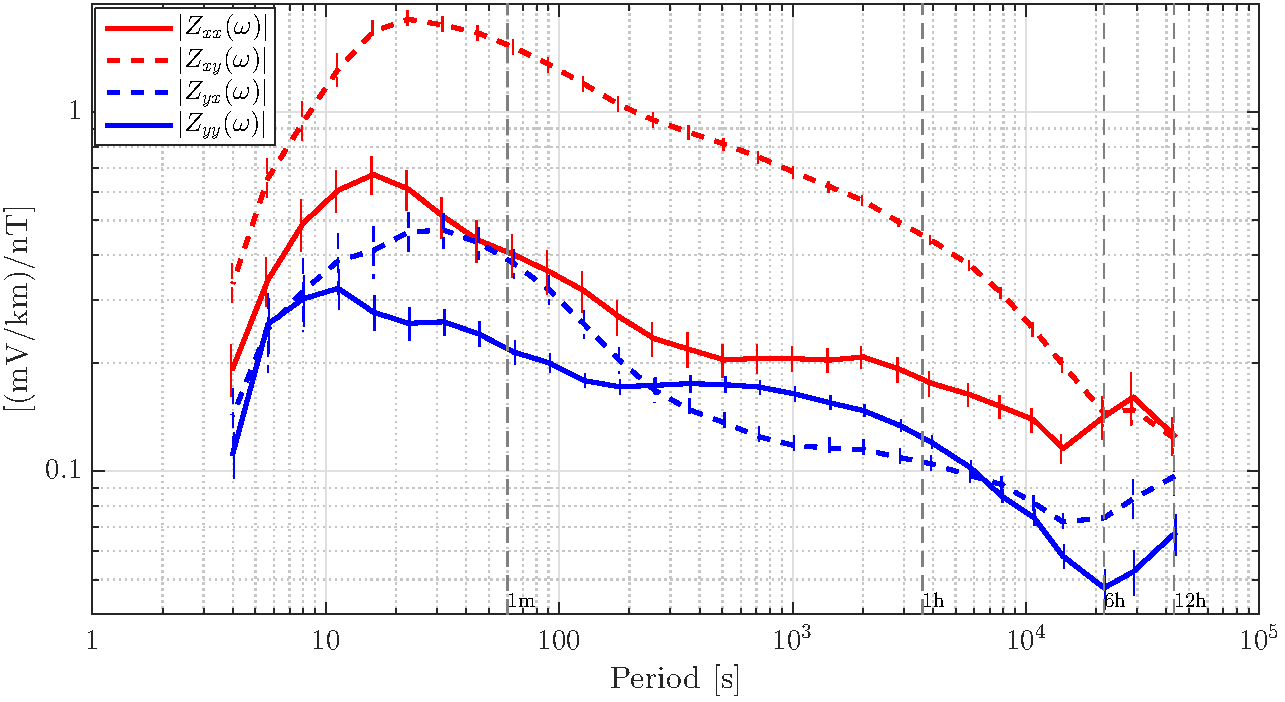
\includegraphics[width=\textwidth]{figures/plot_model_summary_Z_MT-options-1.pdf}
\caption{Frequency domain transfer functions for the parameters in Model~3.}
\label{Z_MT}
%\end{figure}

\vspace{4em}

%\begin{figure}[h]
\centering
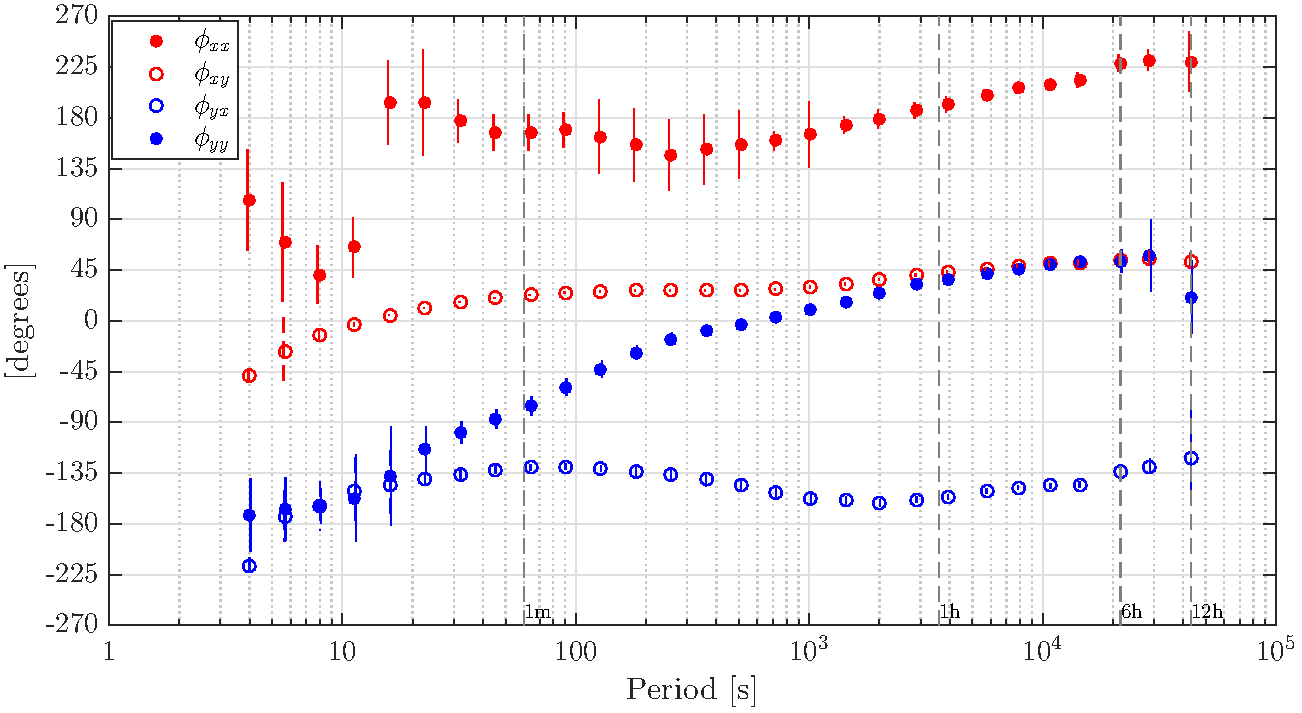
\includegraphics[width=\textwidth]{figures/plot_model_summary_Phi_MT-options-1.pdf}
\caption{Frequency domain phase values for the parameters in Model~3.}
\label{Phi_MT}
\end{figure}

\clearpage

\bibliography{paper.bib}

\end{document}


More Information and Advice:

%% ------------------------------------------------------------------------ %%
%
%  SECTION HEADS
%
%% ------------------------------------------------------------------------ %%

% Capitalize the first letter of each word (except for
% prepositions, conjunctions, and articles that are
% three or fewer letters).

% AGU follows standard outline style; therefore, there cannot be a section 1 without
% a section 2, or a section 2.3.1 without a section 2.3.2.
% Please make sure your section numbers are balanced.
% ---------------
% Level 1 head
%
% Use the \section{} command to identify level 1 heads;
% type the appropriate head wording between the curly
% brackets, as shown below.
%
%An example:
%\section{Level 1 Head: Introduction}
%
% ---------------
% Level 2 head
%
% Use the \subsection{} command to identify level 2 heads.
%An example:
%\subsection{Level 2 Head}
%
% ---------------
% Level 3 head
%
% Use the \subsubsection{} command to identify level 3 heads
%An example:
%\subsubsection{Level 3 Head}
%
%---------------
% Level 4 head
%
% Use the \subsubsubsection{} command to identify level 3 heads
% An example:
%\subsubsubsection{Level 4 Head} An example.
%
%% ------------------------------------------------------------------------ %%
%
%  IN-TEXT LISTS
%
%% ------------------------------------------------------------------------ %%
%
% Do not use bulleted lists; enumerated lists are okay.
% \begin{enumerate}
% \item
% \item
% \item
% \end{enumerate}
%
%% ------------------------------------------------------------------------ %%
%
%  EQUATIONS
%
%% ------------------------------------------------------------------------ %%

% Single-line equations are centered.
% Equation arrays will appear left-aligned.

Math coded inside display math mode \[ ...\]
 will not be numbered, e.g.,:
 \[ x^2=y^2 + z^2\]

 Math coded inside \begin{equation} and \end{equation} will
 be automatically numbered, e.g.,:
 \begin{equation}
 x^2=y^2 + z^2
 \end{equation}


% To create multiline equations, use the
% \begin{eqnarray} and \end{eqnarray} environment
% as demonstrated below.
\begin{eqnarray}
  x_{1} & = & (x - x_{0}) \cos \Theta \nonumber \\
        && + (y - y_{0}) \sin \Theta  \nonumber \\
  y_{1} & = & -(x - x_{0}) \sin \Theta \nonumber \\
        && + (y - y_{0}) \cos \Theta.
\end{eqnarray}

%If you don't want an equation number, use the star form:
%\begin{eqnarray*}...\end{eqnarray*}

% Break each line at a sign of operation
% (+, -, etc.) if possible, with the sign of operation
% on the new line.

% Indent second and subsequent lines to align with
% the first character following the equal sign on the
% first line.

% Use an \hspace{} command to insert horizontal space
% into your equation if necessary. Place an appropriate
% unit of measure between the curly braces, e.g.
% \hspace{1in}; you may have to experiment to achieve
% the correct amount of space.


%% ------------------------------------------------------------------------ %%
%
%  EQUATION NUMBERING: COUNTER
%
%% ------------------------------------------------------------------------ %%

% You may change equation numbering by resetting
% the equation counter or by explicitly numbering
% an equation.

% To explicitly number an equation, type \eqnum{}
% (with the desired number between the brackets)
% after the \begin{equation} or \begin{eqnarray}
% command.  The \eqnum{} command will affect only
% the equation it appears with; LaTeX will number
% any equations appearing later in the manuscript
% according to the equation counter.
%

% If you have a multiline equation that needs only
% one equation number, use a \nonumber command in
% front of the double backslashes (\\) as shown in
% the multiline equation above.

% If you are using line numbers, remember to surround
% equations with \begin{linenomath*}...\end{linenomath*}

%  To add line numbers to lines in equations:
%  \begin{linenomath*}
%  \begin{equation}
%  \end{equation}
%  \end{linenomath*}
